\chapter{Entwurf} \label{chap:entwurf}

\section{Systemarchitektur} \label{sec:systemarchitektur}

In Abbildung \ref{fig:architecture} ist eine grobe Übersicht über die verschiedenen Komponenten des Projektes gegeben.
Es besteht aus drei Komponenten:
\begin{itemize}
	\item Hardware-Tracker
	\item Backend-Anwendung
	\item App
\end{itemize}

Der Hardware-Tracker ist die physische Komponente, die direkt an ein zu trackendes Papier angeheftet wird.
Er wird regelmäßig Daten erfassen und diese zur Lokalisierung an die Backend-Anwendung senden.

Die Backend-Anwendung dient als zentrales Element der Architektur.
Sie bekommt Daten des Trackers zugeschickt, wertet diese aus und speichert sie.
Auch das Management der Räume und Workflows wird von der Anwendung übernommen.

Nutzer verwenden zur Kommunikation mit dem Backend eine Smartphone-App.
Sie kommuniziert ebenfalls mit der Backend-Anwendung und fragt von dieser Informationen an oder löst Aktionen aus.

Die Entwürfe der drei Komponenten werden in den nachfolgenden Abschnitten im Detail erläutert.

\begin{figure}
	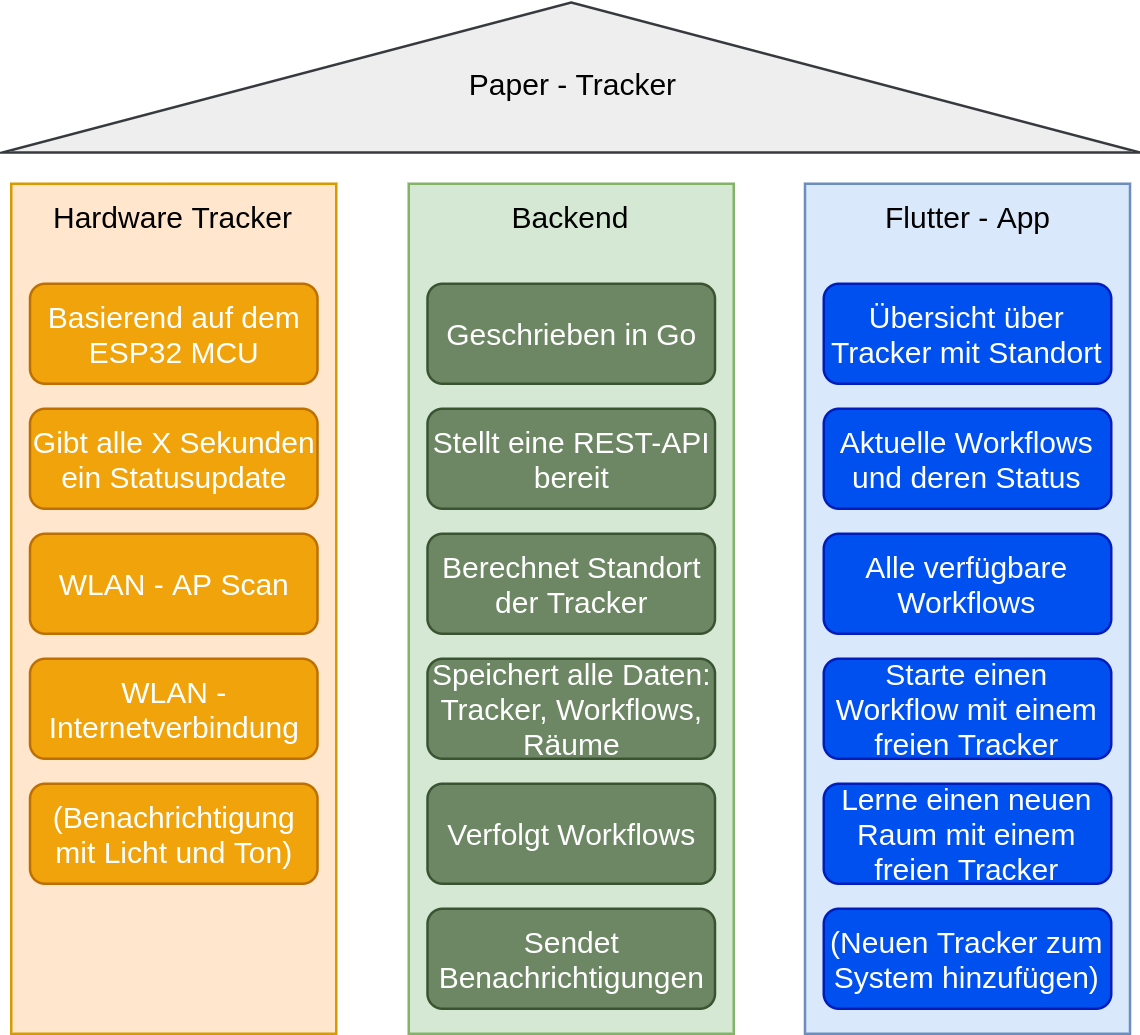
\includegraphics[width=\textwidth]{images/architecture_de.png}
	\centering
	\caption{Architektur des Paper-Tracker}
	\label{fig:architecture}
\end{figure}

\section{Komponentenarchitektur} \label{sec:komponentenarchitektur}

In den folgenden Abschnitten wird detaillierter auf die einzelnen Komponenten des in
\autoref{sec:systemarchitektur} beschriebenen Systems eingegangen.
Dabei werden die Komponenten in derselben Reihenfolge beschrieben, in welcher die Daten im
Gesamtsystem fließen.

\subsection{Tracking mit IoT-Hardware} \label{sec:tracking-hardware}

Zur Erfassung der Standortdaten der Dokumente werden, wie in \autoref{sec:soll-analyse}
beschrieben, Hardware-Tracker eingesetzt.
\TODO{Es wäre schön, Glossar-Referenzen zu kennzeichnen (oft mit Glos, oder Gls)}
Diese verwenden jedoch keine absolute Positionierungstechnologie wie beispielsweise \gls{GPS}, da
das hierfür benötigte Satellitensignal in Gebäuden zu schwach, und somit die Positionierung
fehlschlagen kann.
\TODO{Quelle für die Genauigkeit von GPS in Gebäuden}

\TODO{Ist das hier eher Analyse?}
Für die Lokalisierung von Geräten innerhalb eines Gebäudes gibt es daher mehrere Ansätze.
\TODO{Glossar: Mesh-Netzwerk}
Eine Möglichkeit ist es, ein Mesh-Netzwerk aus den Tracker-Geräten aufzubauen. Ist die Position
einiger weniger Knoten des Meshes bekannt, kann durch die Signalstärke zu umliegenden Knoten oder
über die sogenannte Time-of-Arrival bestimmt werden, wo sich ein Knoten relativ zu anderen Knoten
und damit auch zu den Knoten mit bekannter Position befindet.
\TODO{Time-of-Arrival erläutern}
Mit dieser Methode kann eine Genauigkeit von bis zu einem Meter bei der Lokalisierung erzielt
werden. (vgl. \cite{Patwari2003})

Eine weitere Möglichkeit ist, auf bestehende Infrastruktur zurückzugreifen. \Gls{WLAN} ist
heutzutage in praktisch jedem Gebäude verfügbar.
In Gebäuden, in welchen es mehrere \glspl{AP} gibt, kann die Position dadurch bestimmt werden,
dass der Tracker auswertet, von welchen \glspl{AP} er ein Signal empfängt und wie stark der
Empfang zum jeweiligen \gls{AP} ist.
Da die Positionsdaten ohnehin zur Auswertung an das Backend übertragen werden müssen, wofür eine
\gls{WLAN}-Verbindung notwendig ist, wird diese Methode eingesetzt.
Die gesammelten Daten werden dann im Anschluss an das Backend übermittelt.

\TODO{Lifecycle des Paper-Trackers erläutern}

\subsection{Backend-Anwendung} \label{sec:backend}

\subsubsection{UML Daten Modellierung}
Da die Backend-Anwendung die zentrale Komponente des Systems ist und auch die Daten verwaltet, werden für sie die Daten-Klassen modelliert.
Das resultierende UML-Diagramm ist in Abbildung \ref{fig:uml} abgebildet.

Die zentrale Klasse des Diagramms bildet die \enquote{Tracker}-Klasse.
Sie modelliert einen Hardware-Tracker.
Neben einigen Attributen, wie dem Label, der Batteriestatus und einigen gespeicherten Zeitstempeln, besitzt sie eine Referenz auf einen Status.
Dieser Status gibt an, zu was der Tracker zur Zeit verwendet wird und in welchen anderen Zustand gewechselt werden kann.

Es gibt vier verschiedene Zustände, die in Integern kodiert sind:
\begin{description}
	\item[Idle = 1] \hfill \\
		Tracker ist frei verfügbar und kann in \enquote{Learning} oder \enquote{Tracking} übergehen.
	\item[Learning = 2] \hfill \\
		Tracker wird für das Lernen eines Raumes verwendet und kann bei erfolgreichem Abschluss in \enquote{LearningFinished} oder bei Abbruch in \enquote{Idle} übergehen.
	\item[LearningFinished = 3] \hfill \\
		Das Lernen eines Raumes mit diesem Tracker wurde beendet. Die Ergebnisse können berechnet und einem Raum zugewiesen werden. In Folge darauf, geht der Tracker in den Zustand \enquote{Idle} über.
	\item[Tracking = 4] \hfill \\
		Der Tracker besitzt aktuell einen Workflow, den er trackt. Nach Abschluss dieses Workflows oder nach Abbruch, geht der Tracker in den Status \enquote{Idle} über.
\end{description}

Weiter besitzt der Tracker eine Referenz auf einen aktiven Workflow und den aktuellen Raum.
Beide Referenzen können nichtexistent sein, falls der Tracker keinen aktiven Workflow besitzt oder der Raum nicht bestimmbar ist.

Ein \enquote{Room} ist ein physikalischer Raum, der von einem Tracker erkannt werden soll.
Neben einem Identifizierer und einem \enquote{Label} (Name) für den Raum werden zusätzlich mehrere \enquote{BSSIDTrackingData} gespeichert.
Diese beinhalten für einen spezifischen \enquote{Access Point}/\gls{BSSID} einige Messdaten zu der gemessenen Signalstärke.
Über diese kann über eine Antwort des Trackers mit \enquote{ScanResults} die Position des Tracker bestimmt werden.

Damit der Tracker eine Antwort sendet, wird diese mit Hilfe eines Kommandos angefragt.
Diese Kommandos werden jeweils in einer Instanz der \enquote{Command}-Klasse abgebildet.
Die Kommandos besitzen einen spezifischen Typ der Enumeration \enquote{CommandType}, der die Aktion des Kommandos bestimmt.
Auch wird pro Kommando eine \enquote{SleepTimeSec} festgelegt, die bestimmt wie lange der Tracker sich nach der Aktion abschalten darf.

Spezielle Antworten der Tracker auf Kommandos und auch des Servers auf Anfragen der App sind in dem Unterpaket \enquote{communication} modelliert.
Dies ist zum Beispiel eine Fehler-Antwort und eine Basisklasse für Antworten des Trackers.
Diese \enquote{TrackerResponse}-Klasse besitzt auch ein Feld für den aktuellen Batteriestand des Trackers, um diesen überwachen zu können.

Unter den Klassen \enquote{WorkflowTemplate} und \enquote{WorkflowExec} sind die Workflows modelliert.
\enquote{WorkflowTemplate} stellt eine Blaupause dar, wie ein Workflow aussieht.
In diesem werden die einzelnen Schritte (\enquote{Steps}) des Workflows festgelegt.
Für einen \enquote{Step} werden ein Label und eine Referenz auf den dazugehörigen Raum gespeichert.
Über die Klasse \enquote{NextStep} werden Referenzen auf nachfolgende Schritte modelliert.
Die \enquote{NextStep} Klasse besitzt ein Attribut \enquote{DecisionLabel}.
Ist diese ein leerer String, so ist dieser verbundene Schritt ein linearer.
Mit einem nicht-leeren String, gibt es mit diesem Schritt verschiedene Auswahlmöglichkeiten.
Durch das transitive Attribut \enquote{StepEditingLocked} der \enquote{WorkflowTemplate}-Klasse, wird die Bearbeitung blockiert.
Dieses Attribut ist gesetzt, sobald es eine Ausführung des Templates gab.

Die \enquote{WorkflowExec}-Klasse stellt einen konkreten Workflow in der Durchführung dar.
Als Attribute besitzt diese Klasse ein Label, einen Status und Start-/Endzeit.
Der Status ist entweder \enquote{Running}, \enquote{Completed} oder \enquote{Canceled}.
Weiter besitzt die Klasse eine Referenz auf das Template, das ausgeführt wird, eine Menge an \enquote{ExecStepInfo} und an den aktuellen Schritt.
Die Klasse \enquote{ExecStepInfo} besitzt Informationen über einzelne Schritte des Workflows.
Dies sind zum einen die Start-/Endzeit des Schrittes sowie, ob der Schritt übersprungen wurde, und zum anderen die \enquote{Decision}-Information.
Der \enquote{Decision} String wird im Falle von mehreren Auswahlmöglichkeiten in einem Workflow dazu genutzt, in der Ausführung den richtigen Weg zu wählen.

\begin{figure}
	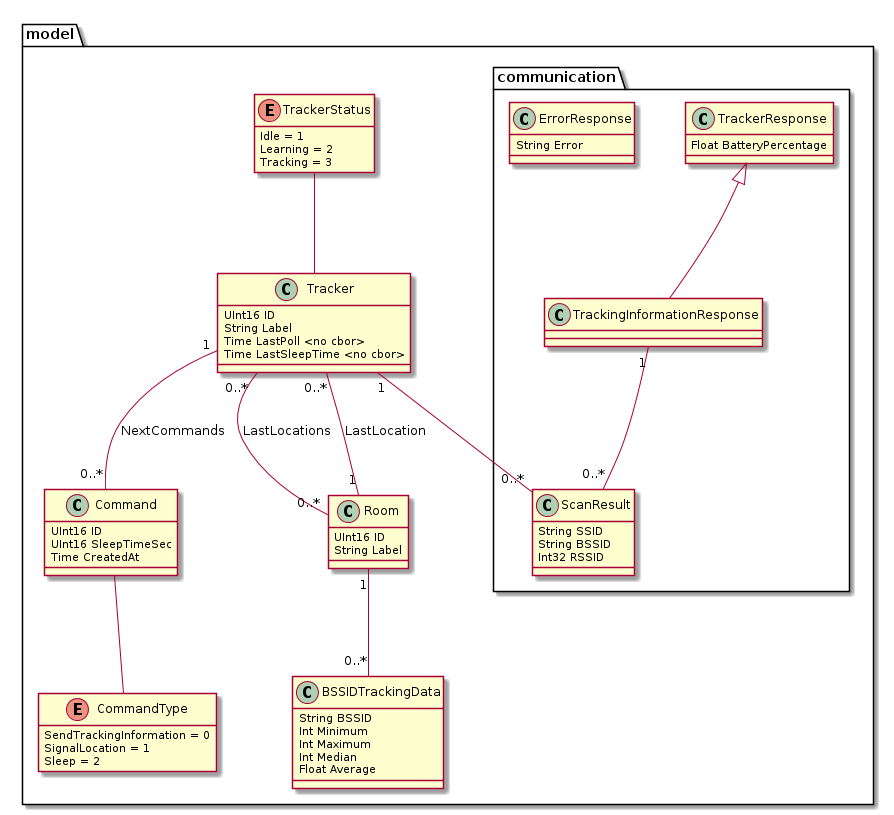
\includegraphics[width=\textwidth]{images/uml.png}
	\centering
	\caption{UML-Diagramm für die Backend-Anwendung}
	\label{fig:uml}
\end{figure}

\FloatBarrier

\subsubsection{Schnittstellen}

Für die Backend-Anwendung sind zwei verschiedene Schnittstellen vorgesehen.
Eine Schnittstelle ist für den Tracker und eine für die App vorgesehen.
Die unterschiedlichen Schnittstellen sollen die aus der Analyse entwickelten Ansprüche entsprechend erfüllen.

\paragraph{Tracker-Schnittstelle}
Für die Schnittstelle des Trackers bedeutet dies, dass sie möglichst simpel und effizient sein muss.
Dies wird über ein entsprechendes Protokoll und einem Datenformat erreicht.
Das verwendete Protokoll ist das \acrfull{CoAP} Protokoll und das Datenformat ist \acrfull{CBOR}.

Bei \gls{CoAP} handelt es sich um ein spezialisiertes Protokoll für die Verwendung in
\gls{IoT}-Hardware, welches dafür optimiert wurde möglichst wenig \gls{Overhead} zu haben.

Im \gls{IoT}-Bereich haben sich einige Protokolle durchsetzen können. Dazu zählen vor allem
\gls{HTTP}, \gls{MQTT}, \gls{AMQP} und \gls{CoAP}.
Da die Tracker batteriebetrieben sind, ist für diesen Anwendungsfall besonders die Performance des
eingesetzten Protokolles wichtig. Je weniger Overhead das Protokoll aufweist, desto weniger
Instruktionen müssen vom Prozessor des Trackers durchgeführt werden, was zu einer längeren Laufzeit
führt.
Werden die Protokolle anhand dieses Aspektes verglichen, erweist sich \gls{CoAP} als effizientestes
Protokoll. (vgl. \cite{Dizdarevic2019}, \cite{Naik2017})
\TODO{Quellen verwenden, die in diesem Paper zitiert werden}

\gls{CBOR} ist ein Datenformat, das auf kleine Code- und Nachrichtengrößen optimiert ist.
Demnach ist es auch für der \gls{IoT}-Bereich sehr gut geeignet.
Vom Aufbau des Formats, ist es sehr gut mit \gls{JSON} zu vergleichen, da es auch Schlüssel-Wert-Paare verwendet.
Der große Unterschied ist jedoch, dass \gls{CBOR} binär kodiert wird und \gls{JSON} in Text kodiert wird.
Dadurch ist \gls{CBOR} nicht menschenlesbar aber sehr gut maschinenlesbar.
Bei einem Vergleich zwischen der \gls{CBOR} Bibliothek \enquote{libCBOR} und der \gls{JSON} Bibliothek \enquote{ArduinoJson}
konnte zudem festgestellt werden, dass bei gleicher Nachricht das \gls{CBOR} Format ca. 26.5\% kleinere Nachrichten
in 83.3\% der Zeit schnellerer Zeit serialisiert hat.

\TODO{Hier das Polling-Prinzip oder unter Hardware?!}

Die Tracker-Schnittstelle soll drei Endpunkte zur Verfügung stellen.
Diese sind in \autoref{tab:coap-api} aufgelistet.
Bis auf den Endpunkt zum erstellen eines neuen Trackers, erhalten alle Endpunkte als Parameter die Tracker ID des Trackers, der die Anfrage stellt.
Der Endpunkt zum Speichern der Tracking Ergebnisse hat zudem als Parameter die Ergebnisste selbst.

\begin{table}[]
\begin{tabular}{l|l|l|l}
\textbf{Verb} & \textbf{Pfad}     & \textbf{Aktion}                   & \textbf{Rückgabe-Wert}    \\ \hline
POST          & /tracker/new      & Neuen Tracker erstellen           & Tracker ID \\ \hline
GET           & /tracker/poll     & Kommando für Tracker abfragen     & Tracker Kommando   \\ \hline
POST          & /tracker/tracking & Ergebnisse des Tracking speichern & -
\end{tabular}
\caption{\label{tab:coap-api}Verfügbare Endpunkte der Tracker-Schnittstelle}
\end{table}

\FloatBarrier
\paragraph{App-Schnittstelle}
Die Schnittstelle für die App hat keine besonderen Anforderungen und kann daher frei gewählt werden.
Aus diesem Grund werden Protokolle und Datenformate verwendet, die momentan dem aktuellen Stand der
Technik entsprechen. \TODO{Quelle für aktuelle Protokolle}
Dies ergibt den Vorteil, dass sie mit allen anderen gewählten Technologien sehr gut kombinierbar sind und entsprechende Bibliotheken vorhanden sind.
Das verwendete Protokoll ist das \gls{HTTP}-Protokoll und das Datenformat ist \gls{JSON}.
Die Schnittstelle basiert auf dem \gls{REST} Paradigma. \TODO{Soll REST erläutert werden?}
Alle verfügbaren Endpunkte der App-Schnittstelle sind in \autoref{tab:http-api} dargestellt.

\TODO{Zwischen"überschriften" hinzufügen für Room, Tracker, etc.}
\TODO{Erläuterung der einen Abkürzung (wf)?}
\FIXME{Hinzufügen einer caption führt zu Fehlern}
\begin{small}
\begin{landscape}
	\begin{longtable}{l|l|l|l|l} \label{tab:http-api}
\textbf{Verb} & \textbf{Pfad}                   & \textbf{Aktion}                     & \textbf{Parameter}                                          & \textbf{Rückgabe-Wert}                                                  \\ \hline
\endhead
%
GET           & /room                           & Auflistung der Räume                & -                                                           & Liste aller Räume                                                       \\ \hline
POST          & /room                           & Erstellen eines neuen Raums         & Raum                                                        & Erstellter Raum                                                         \\ \hline
PUT           & /room/:id                       & Raum aktualisieren                  & Raum                                                        & Aktualisierter Raum                                                     \\ \hline
DELETE        & /room/:id                       & Raum löschen                        & -                                                           & -                                                                       \\ \hline
GET           & /tracker                        & Auflistung der Tracker              & -                                                           & List aller Tracker                                                      \\ \hline
PUT           & /tracker/:id                    & Tracker aktualisieren               & Tracker                                                     & Aktualisierter Tracker                                                  \\ \hline
DELETE        & /tracker/:id                    & Tracker löschen                     & -                                                           & -                                                                       \\ \hline
POST          & /tracker/:id/learn              & Lernen mit Tracker starten          & -                                                           & Lernzeit                                                                \\ \hline
GET           & /tracker/:id/learn              & Lern Status abfragen                & -                                                           & \begin{tabular}[c]{@{}l@{}}Abgeschlossen\\ Gefundene SSIDs\end{tabular} \\ \hline
DELETE        & /tracker/:id/learn              & Lernen abbrechen                    & -                                                           & -                                                                       \\ \hline
POST          & /tracker/:id/learn/finish       & Lernen abschließen                  & \begin{tabular}[c]{@{}l@{}}Raum ID\\ SSIDs\end{tabular}     &                                                                         \\ \hline
GET           & /workflow/template              & Auflistung der Templates            & -                                                           & Liste aller Templates                                                   \\ \hline
POST          & /workflow/template              & Template erstellen                  & Template                                                    & Erstelltes Template                                                     \\ \hline
PUT           & /workflow/template/:id          & Template aktualisieren              & Tempalte                                                    & Aktualisiertes Template                                                 \\ \hline
DELETE        & /workflow/template/:id          & Template löschen                    & -                                                           & -                                                                       \\ \hline
POST          & /workflow/template/:id/start    & Start Schritt erstellen             & Step                                                        & Erstellter Step                                                         \\ \hline
POST          & /workflow/template/:id/step     & Schritt hinzufügen                  & \begin{tabular}[c]{@{}l@{}}Step\\ Vorgänger ID\end{tabular} & Erstellter Step                                                         \\ \hline
GET           & /workflow/template/:id/step/:id & Schritt abfragen                    & -                                                           & Step                                                                    \\ \hline
PUT           & /workflow/template/:id/step/:id & Schritt aktualisieren               & Step                                                        & Aktualisierter Step                                                     \\ \hline
DELETE        & /workflow/template/:id/step/:id & Schritt löschen                     & -                                                           & -                                                                       \\ \hline
POST          & /wf/template/:id/step/:id/move  & Schritt verschieben                 & Richtung                                                    & -                                                                       \\ \hline
POST          & /workflow/template/revision     & Template Revision erstellen         & Label                                                       & Erstellte Revision                                                      \\ \hline
GET           & /workflow/exec                  & Auflistung der Ausführungen         & -                                                           & Execution                                                               \\ \hline
POST          & /workflow/exec                  & Ausführung erstellen                & Execution                                                   & Erstelle Execution                                                      \\ \hline
POST          & /workflow/exec/:id/progress/:id & Ausführung zu Schritt progressieren & -                                                           & -                                                                       \\ \hline
POST          & /workflow/exec/:id/cancel       & Ausführung abbrechen                & -                                                           & -
\end{longtable}
\end{landscape}
\end{small}

\subsection{App für Mobilgeräte} \label{sec:app}

